\documentclass{beamer}
\usepackage{amsmath}
\usepackage{xcolor}
\usepackage{multimedia}
\usetheme{copenhagen}
\definecolor{purple}{rgb}{0.3,0,0.4}
\definecolor{aqua}{rgb}{0,0.85,0.8}
\definecolor{grey}{rgb}{60,60,60}
\setbeamercolor*{palette primary}{use=structure, fg=white, bg=purple}
\setbeamercolor*{background canvas}{bg=purple!5}
\setbeamercolor*{block title example}{use=structure,fg=white,bg=purple}
\setbeamercolor*{block body example}{fg=black,use=block title,bg=purple!20}
\setbeamercolor*{block title}{use=example text,fg=white,bg=aqua!60!black}
\setbeamercolor*{block body}{fg=black,use=block title example,bg=aqua!10}

\usepackage{graphicx}
\usepackage{tikz-cd}

\newcommand{\Gal}{\mathrm{Gal}}
\newcommand{\Cl}{\mathrm{Cl}}

\newcommand{\CC}{\mathbb{C}}
\newcommand{\FF}{\mathbb{F}}
\newcommand{\NN}{\mathbb{N}}
\newcommand{\PP}{\mathfrak{P}}
\newcommand{\QQ}{\mathbb{Q}}
\newcommand{\RR}{\mathbb{R}}
\newcommand{\ZZ}{\mathbb{Z}}
\newcommand{\GG}{\mathbb{G}}
\newcommand{\adele}{\mathbb{A}}
\newcommand{\pp}{\mathfrak{p}}
\newcommand{\qq}{\mathfrak{q}}
\newcommand{\rr}{\mathfrak{r}}
\newcommand{\af}{\mathfrak{a}}

\theoremstyle{plain}
\newtheorem{thm}{Theorem}[section]
\newtheorem{rem}[thm]{Remark}
\newtheorem{proposition}[thm]{Proposition}
\newtheorem{conjecture}[thm]{Conjecture}



\graphicspath{ }


\title{The Generalized Fermat Equation}
\author{Albert Lopez Bruch}
%\institute{LSGNT}
\date{17 October, 2024}

\begin{document}

\frame{\titlepage}


\begin{frame}
    \frametitle{Introduction -- Pythagorean Triples}
    Initial question: Which right triangles have integer-valued sides?
    Eight centuries after Pythagoras, Diophantus first phrased this question as solutions to the equation
    \begin{equation}\label{pythragoras}
        x^2+y^2=z^2, \quad\text{with}\ x,y,z\in\NN \text{ and }\gcd(x,y,z)=1.
    \end{equation}

    \begin{theorem}[Diophantus, 3rd C.]
        The solutions to \eqref{pythragoras} are given by
        \[\{x,y\}=\{2mn,m^2-n^2\},\quad z=m^2+n^2,\]
        where $m\geq n$ are positive integers.
    \end{theorem}
    \begin{proof}
        One factorizes $z^2=(x+iy)(x-iy)$ and observes that $\gcd(x+iy,x-iy)=1$. Since $\ZZ[i]$ is a UFD, $x+iy=u(m+in)^2$, where $u\in\{\pm1,\pm i\}$ is a unit in $\ZZ[i]$ and $m,n\in\ZZ$.
    \end{proof}
\end{frame}

\begin{frame}
    \frametitle{Introduction -- The Fermat Equation}
    Diophantus' work was lost for centuries, and it wasn't until 1634 when Fermat conjectured that the equation
    \begin{equation}\label{fermat}
        x^n+y^n=z^n, \quad\text{with}\ x,y,z\in\NN \text{ and }\gcd(x,y,z)=1.
    \end{equation}
    has no solutions for $n\geq 2$, known as Fermat's Last Theorem (FLT). This statement evaded mathematicians for 3 centuries and sparked enormous development. Attempts included
    \begin{itemize}
        \item Infinite descent.
        \item Understanding of cyclotomic fields.
        \item Analytic methods.
        \item Modularity and Galois representations.
    \end{itemize}    
    \begin{theorem}[Wiles, 1994]
        The only integer solutions to \eqref{fermat} satisfy $xyz=0$. 
    \end{theorem}
\end{frame}


\begin{frame}
    \frametitle{The Generalized Fermat Equation}
    Even before Wiles' proof, various authors had studied equations of the shape
    $$Ax^p+By^q=Cz^r,\quad \text{ for fixed }A,B,C.$$
    Today we focus on the equation
    \begin{equation}\label{generalized}
        x^p+y^q=z^r, \quad\text{with}\ x,y,z\in\NN \text{ and } \gcd(x,y,z)=1.
    \end{equation}
    Let $\sigma(p,q,r)=1/p+1/q+1/r$ be the signature of \eqref{generalized}, and one distinguishes the cases:
    \begin{enumerate}
        \item Spherical case if $\sigma(p,q,r)>1$.
        \item Parabolic case if $\sigma(p,q,r)=1$.
        \item Hyperbolic case if $\sigma(p,q,r)<1$.
    \end{enumerate}
\end{frame}

\begin{frame}
    \frametitle{Spherical Case}
    In this case, if $\sigma(p,q,r)>1$, then $(p,q,r)$ is one of $(2,2,r)$, $(2,q,2)$, $(2,3,3)$, $(2,3,4)$, $(2,3,5)$ or $(2,4,3)$. 
    \begin{theorem}
        If $\sigma(p,q,r)>1$, then $$x^p+y^q=z^r$$ has infinitely many solutions, and they come in finitely many two-parameter families.
    \end{theorem}
    The proof is purely elementary, relying heavily on the parametrization of pythagorean-related equations.
    
\end{frame}

\begin{frame}
    \frametitle{Spherical Case}
    \begin{example}
        The solutions to $x^2+y^4=z^3$ come in four families, one of which is
        \[
        \begin{cases}
            x=4ts(s^2-3t^2)(s^4+6t^2s^2+81t^4)(3s^4+2t^2s^2+3t^4),\\
            y=\pm(s^2+3t^2)(s^4-18t^2s^2+9t^4),\\
            z=(s^4-2t^2s^2+9t^4)(s^4+30t^2s^2+9t^4)
        \end{cases}
        \]
        where $\gcd(s,t)=1$, $s\not\equiv t\pmod2$ and $3\nmid s$.
    \end{example}
    \begin{example}
        The solutions to $x^2+y^3=z^5$ come in $27$ distinct families. 
    \end{example}
\end{frame}


\begin{frame}
    \frametitle{Parabolic Case}
    If $\sigma(p,q,r)=1$, then $$(p,q,r)=(2,3,6),\ (2,4,4),\ (2,6,3),\ (3,3,3)\text{ or }(4,4,2).$$
    
    %Infinite descent gives a way to prove that no solutions exist for some of these cases.
    \begin{proof}[Fermat: $(4,4,2)$ case]
        Suppose that $x^4+y^4=z^2$ is a non-trivial solution with $x$ odd and minimal $z$. Then 
        $$x^2=m^2-n^2,\quad y^2=2mn,\quad z=m^2+n^2,$$
        and since $(x,n,m)$ is also a pythagorean triple,
        $$x=r^2-s^2,\quad n=2rs,\quad m=r^2+s^2$$
        for coprime $r,s$, also pairwise coprime with $m$. From $y^2=4mrs$, we obtain that $r=a^2$, $s=b^2$, $m=c^2$ giving $a^4+b^4=c^2,$ a contradiction.
    \end{proof}

\end{frame}


\begin{frame}
    \frametitle{Parabolic Case}
    The parabolic case is completely solved.
    \begin{theorem}
        The only primitive non-trivial solution of the parabolic case comes from the signature $(p,q,r)=(2,3,6)$ and corresponds to the solution $3^2=2^3+1$.
    \end{theorem}
    Each equation corresponds to an elliptic curve over $\QQ$ of rank $0$.
    \begin{example}[Signature $(3,3,3)$]
        The equation $x^3+y^3=z^3$ can be transformed to $E:Y^2=X^3-432.$ %by the transformation 
        %$$Y=\frac{36(x-y)}{x+y},\quad X=\frac{12z}{x+y}.$$
        One can then show that 
        $$E(\QQ)=\{\mathcal{O},(36,12),(36,-12)\}\cong\ZZ/3\ZZ,$$
        giving the trivial solutions $[1:-1:0], [1:0:1], [0:1:1]$.
    \end{example}
\end{frame}

\begin{frame}
    \frametitle{Parabolic Case}
    \begin{example}[Signatures $(2,3,6)$ and $(2,6,3)$]
        The equation $x^3\pm y^6=z^2$ can be transformed to $$E^{\pm}:Y^2=X^3\pm1.$$ One then shows that $E^-(\QQ)=\{\mathcal{O},(1,0)\}\cong\ZZ/2\ZZ$, while
        $$E^+(\QQ)=\{\mathcal{O},(-1,0),(0,\pm1),(2,\pm 3)\}\cong\ZZ/6\ZZ.$$
        The points $(2,\pm 3)$ give rise to the unique solutions $(x,y,z)=(2,\pm1,\pm3)$.
    \end{example}
\end{frame}

\begin{frame}
    \frametitle{Hyperbolic Case}
    %From now on, we consider the equation
    %\begin{equation}\label{hyperbolic}
        %x^p+y^q=z^r,\text{ with } x,y,z\in\NN,\gcd(x,y,z)=1\text{ and }\frac{1}{p}+\frac{1}{q}+\frac{1}{r}<1.
    %\end{equation}
    From now on, we consider the \textit{hyperbolic} case $\sigma(p,q,r)<1$. Currently, we know the solutions $1^p+2^3=3^2$ and 
    \begin{figure}
        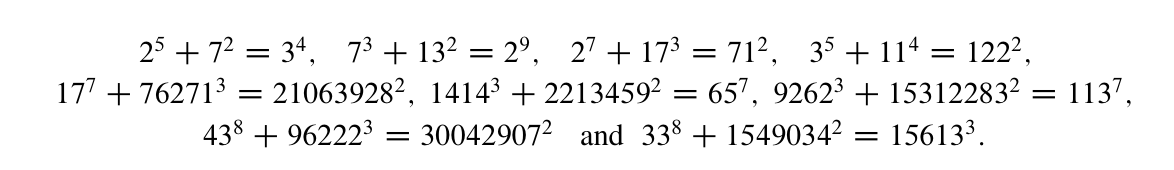
\includegraphics[scale=0.34]{beal_examples.png}
    \end{figure}
    \begin{conjecture}[Beal, 1993]
        There are no non-trivial solutions of $x^p+y^q=z^r$ if $1/p+1/q+1/r<1$ and $\min\{p,q,r\}\geq 3$.
    \end{conjecture}
    A prize of one million dollars is awarded for the solution!
    
    To analyze the progress on this conjecture, we need to look to the cyclotomic and modular approach to FLT. 
\end{frame}


\begin{frame}
    \frametitle{Hyperbolic Case}
    \begin{theorem}[Darmon, Granville, 1995]
        If $A,B,C,p,q,r$ are fixed positive integers with
        $1/p+1/q+1/r<1,$
        then the equation 
        $$Ax^p+By^q=Cz^r$$
        has finitely many solutions in coprime non-zero integers $x,y,z$.
    \end{theorem}
    \begin{proof}[Proof sketch]
        One uses $1/p+1/q+1/r<1$ to show the existence of a cover $\phi:D\to\mathbb{P}^1$ such that $D$ has genus $\geq 2$ and
        \begin{itemize}
            \item It is only ramified above $0,1,\infty$.
            \item All ram degrees above $0,1,\infty$ divide $p,q,r$ respectively.
        \end{itemize}
        If $(x,y,z)$ is a solution, $\phi^{-1}(Ax^p/Cz^q)$ is defined over a number field $K$ unramified away from $2ABCpqr$. Now apply Hermite and Falting's theorem.
    \end{proof}
\end{frame}


\begin{frame}
    \frametitle{Fermat-Catalan Equation and Cyclotomic Approach}
    We now consider the Fermat-Catalan equation
    $$x^p+y^p=z^q,\quad\text{with}\ x,y,z\in\NN\text{ and }\gcd(x,y,z)=1.$$
    We may assume that $p$ and $q$ are prime, and we consider:
    \begin{enumerate}
        \item FLT$(p,q)$1 if $p\nmid xyz$. Then
        $$z^q=(x+y)\prod_{c=1}^{p-1}(x+y\zeta_p^c)$$
        \item FLT$(p,q)$2 if $p\mid xyz$. Then, if $p\mid z$,
        $$z^q=p(x+y)\prod_{c=1}^{p-1}\left(\frac{x+y\zeta_p^c}{1-\zeta_p}\right)$$
    \end{enumerate}

\end{frame}


\begin{frame}
    \frametitle{Fermat-Catalan Equation and Cyclotomic Approach}
    \begin{enumerate}
        \item FLT$(p,q)$1 if $p\mid xyz$. Then
        $$z^q=(x+y)\prod_{c=1}^{p-1}(x+y\zeta_p^c)$$
        \item FLT$(p,q)$2 if $p\mid xyz$. Then, if $p\nmid z$,
        $$z^q=p(x+y)\prod_{c=1}^{p-1}\left(\frac{x+y\zeta_p^c}{1-\zeta_p}\right)$$
    \end{enumerate}
    If $K=\QQ(\zeta_p)$, then $\mathcal{O}_K=\ZZ[\zeta_p]$ and $\alpha=\frac{x+y\zeta_p}{(1-\zeta_p)^e}$ satisfies 
    \begin{equation}
        (\alpha)=\mathfrak{A}^q\quad\text{and}\quad N_{K/\QQ}(\alpha)=\frac{z^q}{p^e(x+y)}
    \end{equation}
    where $\mathfrak{A}$ is an ideal of $K$.
\end{frame}

\begin{frame}
    %\frametitle{Cyclotomic Approach}
    Arithmetic understanding of $\QQ(\zeta_p)$ together with analytic methods has given remarkable progress.
    \begin{theorem}[Kummer]
        FLT holds for regular primes (i.e primes $p$ such that $p\nmid \mathrm{Cl}(\QQ(\zeta_p))$)        
    \end{theorem} 
    \begin{theorem}[Granville, Monagan]
        If FLT1 has a non-trivial solution, then 
        $$a^{p-1}\equiv1\pmod{p^2}\quad\text{for }a\in\{2,3,\ldots,89\}$$        
    \end{theorem}
    Corollary: FLT1 has no solutions for $p<714,591,416,091,389$
    \begin{theorem}[Mihailescu, 2001]
        The only non-trivial solution of the Catalan equation
        $$x^p-y^q=1$$
        comes from $3^2-2^3=1$.
    \end{theorem}

\end{frame}

\begin{frame}
    \frametitle{Fermat's Last Theorem}
    To prove more results about Beal's conjecture, one looks at the main ideas leading to the proof of FLT. Here are the main pillars:
    \begin{enumerate}
        \item Mazur’s Theorem on irreducibility of Galois representations of elliptic curves;
        \item The modularity theorem, due to Wiles, Breuil, Conrad, Diamond and Taylor;
        \item Ribet’s level lowering theorem.
    \end{enumerate}
\end{frame}




\begin{frame}
    \frametitle{Galois Representations}
    Let $E$ be an elliptic curve over $\QQ$ and let $p$ be a prime. Since the $p$-torsion satisfies $E[p]\cong(\ZZ/p\ZZ)^2$ and has algebraic coordinates, we has a mod $p$ Galois representation
    \[\bar{\rho}_{E,p}:\Gal(\bar\QQ/\QQ)\longrightarrow\mathrm{GL}_2(\FF_p).\] 
    \begin{theorem}[Mazur, 1978]
        \begin{itemize}
            \item Let $E$ be an elliptic curve over $\QQ$ and $p>163$ a prime. Then $\bar\rho_{E,p}$ is irreducible.
            \item Let $E$ be an elliptic curve over $\QQ$ with $E[2]\subseteq E(\QQ)$ and $p\geq 5$ a prime. Then $\bar\rho_{E,\rho}$ is irreducible.  
        \end{itemize}
    \end{theorem}
    Mazur's Theorem is equivalent to the statement that any elliptic curve over $\QQ$ has no $p$-isogenies for $p>163$.
\end{frame}



\iffalse
\begin{frame}
    \frametitle{The Modularity Theorem}
    A modular form $f$ of weight $k$ and level $N$ has a Fourier expansion $$f(z)=\sum_{n\geq 0}c_nq^n,$$
    and we denote this space as $M_k(N)$. The space of cusps forms, with $c_n=0$, is denoted $S_k(N)$. We now focus on weight $k=2$, and recall there is a family of commuting operators
    $$T_n:S_2(N)\longrightarrow S_2(N)$$
    An eigenform $f\in S_n(N)$ is a simultaneous eigenvalue for all $T_n$, and it is normalized if $c_1=1$.

\end{frame}
\fi

\begin{frame}
    \frametitle{The Modularity Theorem}
    Let $S_2(N)$ be the space of weight $k=2$ and level $N$ cusp forms. There is a family of commuting operators
    $$T_n:S_2(N)\longrightarrow S_2(N),$$
    An eigenform $f$ is a simultaneous eigenvalue for all $T_n$, and it is normalized if $c_1=1$.

    \begin{theorem}[The Modularity Theorem]
    Let $E$ be an elliptic curve over $\QQ$ with conductor $N$. There exists a normalized eigenform $f=q+\sum c_nq^n$ of weight $2$ and
    level $N$ such that $c_n\in\ZZ$, and if $p\nmid\Delta_E$ is prime then $c_p=a_p(E)=p+1-|\tilde{E}(\FF_p)|$.
    \end{theorem}

\end{frame}
    
\begin{frame}
    \frametitle{Ribet’s Level Lowering Theorem}
    Given an eigenform $f\in S_2(N)$ and a prime $p$, we can associate
    $$\bar\rho_{f,p}:\Gal(\bar\QQ/\QQ)\longrightarrow \mathrm{GL}_2(\FF_{p^r}),$$
    where $r\geq1$ depends on $f$ (and $r=1$ if and only if all $c_n\in\ZZ$). 
    \textbf{Fact:} $\bar\rho_{E,p}\sim\bar\rho_{f,p}$ if $E$ corresponds to $f$.
    \begin{theorem}[Ribet’s Level Lowering Theorem, 1986]
        Let $E$ be an elliptic curve over $\QQ$ with minimal discriminant $\Delta$ and conductor $N$ and let $p\geq3$ be prime. Suppose
        \begin{itemize}
            \item the curve $E$ is modular;
            \item the mod $p$ representation $\bar\rho_{E,p}$ is irreducible
        \end{itemize}
        Let $$N_p=N\big/\prod_{\substack{\ell\mid N\\p\mid\mathrm{ord}_\ell(\Delta)}}\ell.$$
        Then $\bar\rho_{E,p}\sim\bar\rho_{g,p}$ for some eigenform $g$ of weight $2$ and level $N_p$.
    \end{theorem}

\end{frame}

\begin{frame}
    \frametitle{Proof of Fermat's Last Theorem}
    Suppose that $(x,y,z)$ is a non-trivial solution of $x^p+y^p=z^p$ for $p\geq5$. Reorder them so that $y$ is even and $x^p\equiv-1\pmod{4}$. Define the \textbf{Frey–-Hellegouarch curve} $$E:Y^2=X(X-x^p)(X+y^p)$$ with $$\Delta=x^{2p}y^{2p}z^{2p}2^{-8}\quad\text{and}\quad N=\prod_{\ell\mid\Delta}\ell.$$
    We have that $E$ is modular and since $E[2]\subseteq E(\QQ)$ and $p\geq5$, the representation $\bar\rho_{E,p}$ is irreducible. So Ribet's Theorem applies and $N_p=2$. This predicts the existence of some eigenform $g\in S_2(2)$. However, $\dim S_2(2)=g(X_0(2))=0$, so no non-trivial solution can exist.\qed

\end{frame}

\begin{frame}
    \frametitle{How much do we know?}
    \begin{figure}
        \centering
        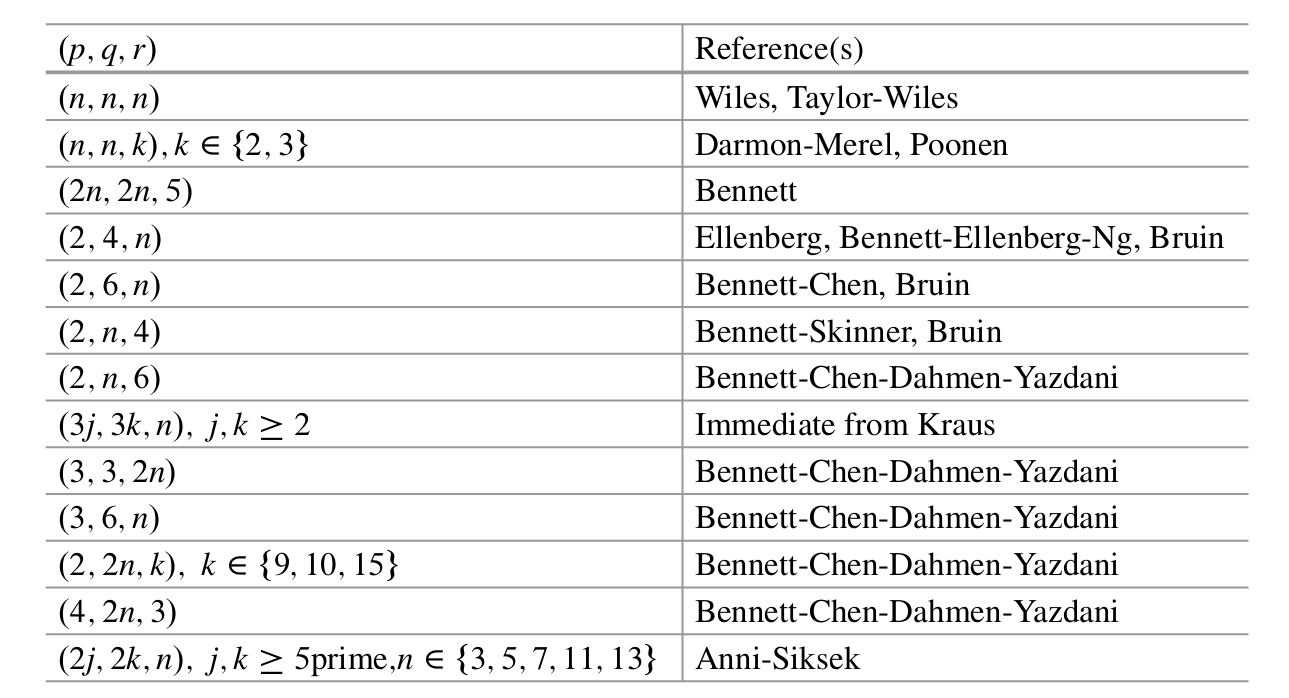
\includegraphics[scale=0.3]{known1.png}
        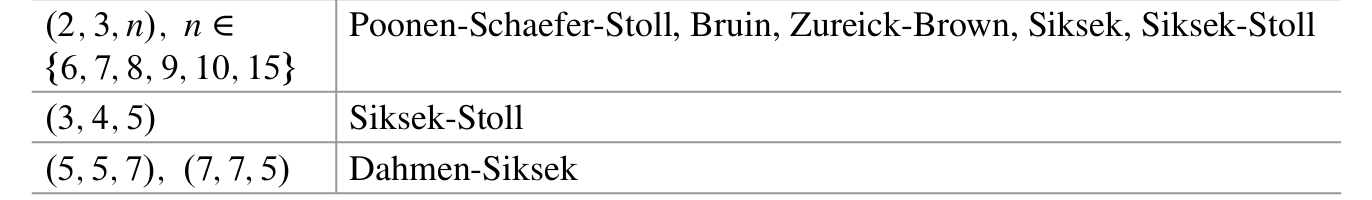
\includegraphics[scale=0.282]{known2.png}
    \end{figure}

\end{frame}

\begin{frame}
    \frametitle{How much do we know?}
    Essentially two methods of proof:
    \begin{itemize}
        \item For some fixed triples, the problem is reduced to finding $\QQ$-rational points on curves of genus $\geq2$.
        \item Using \textit{Frey–-Hellegouarch curves} associated to $(p,q,r)$: elliptic curves $E/\QQ$ attached to a solution such that
        \begin{enumerate}
            \item $\Delta=A\cdot B^p$ where $A$ is a known small integer;
            \item every prime $p\mid B$ divides the conductor exactly once.
        \end{enumerate}
    \end{itemize}
    \begin{figure}
        \centering
        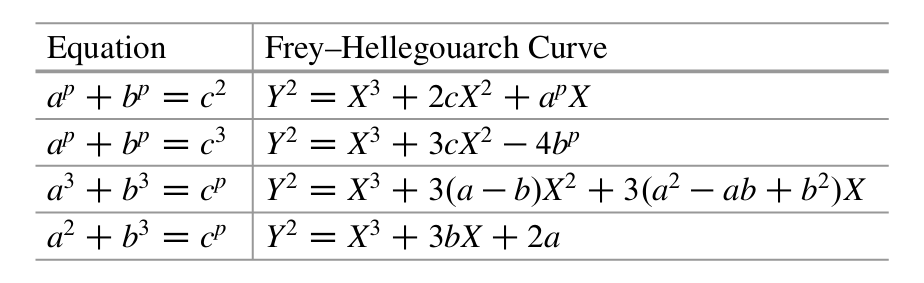
\includegraphics[scale=0.4]{fh_curves.png}
    \end{figure}
    
\end{frame}


\begin{frame}
    \frametitle{}

\end{frame}


\begin{frame}
    \frametitle{}

\end{frame}

\begin{frame}
    \frametitle{}

    
\end{frame}


\begin{frame}
    \frametitle{}

\end{frame}


\begin{frame}
    \frametitle{}

\end{frame}


\begin{frame}
    \frametitle{}
     
\end{frame}


\begin{frame}
    \frametitle{}

\end{frame}


\begin{frame}
    \frametitle{}


\end{frame}


\begin{frame}

\end{frame}


\begin{frame}
    Thank you for listening!
\end{frame}

\end{document}